\lab{Algorithms}{Complex Numbers}{Complex Numbers}
\label{Lab:complex_intro}

\objective{Learn to perform basic computation and visualization with complex numbers.}

\section*{Arithmetic with complex numbers}
Computationally, complex numbers are really just a pair of floating point numbers.
The first is understood to represent the real part of the complex number.
The second is understood to represent the imaginary part.
In Python, a complex number $a + b i$ can be defined using either of the following methods
\begin{lstlisting}
complex(a, b)
a + 1.0j * b
\end{lstlisting}
Python lets us define purely imaginary numbers using the syntax shown there with \li{j}.
As another example, $2 i$ would be \li{2.0j}.

Python also includes the built in \li{cmath} library.
This library provides basic math functions for complex numbers.
For examle, the functions \li{polar} and \li{rect} can be used to convert to and from polar coordinates (discussed below).
It also includes basic functions like \li{sin}, \li{cos}, etc. with their domains extended to the complex numbers.

There are some computational advantages and disadvantages to using complex numbers.
Addition or subtraction between two complex numbers now requires two floating point operations (one for each part of the number), so it takes longer.
Multiplication and division are more costly.
Mutliplication is easily seen to take 4 floating point multiplies and two floating point adds instead of just a single floating point multiply.
The fact that there two numbers are stored also increases the amount of floating point error that can be created in each computation.

Most of the basic functions in NumPy support complex numbers.
Fore example, \li{numpy.absolute} will take the absolute value of a complex number without any trouble.
You can also acces the real and imaginary parts of a complex array via the \li{real} and \li{imag} attributes.
For example,
\begin{lstlisting}
import numpy as np
from numpy.random import rand
Z = rand(10) + 1.0j * rand(10)
# print real part
print Z.real
# print imaginary part
print Z.imag
\end{lstlisting}

The complex conjugate of a complex number or array can be obtained using the \li{conjugate} method.
For example, if \li{A} is a complex number or complex array, its conjugate (or elementwise conjugate) is obtained via
\begin{lstlisting}
A.conjugate()
\end{lstlisting}

\section*{Polar Representation of Complex Numbers}

One of the most important results in Complex Analysis is Euler's Formula.
It states that:

\[e^{i\theta}=cos(\theta)+i sin(\theta)\]

One way to derive this important result is to consider the taylor series expansion of each of the functions involved.

From this formula, we can see that $e^x$ maps the imaginary axis onto the unit circle on the complex plane.
From our knowledge of the sine and cosine functios, we can also know that this mapping has a period of $2\pi$.
From here, notice that we may represent any number on the complex plane in the form $r e^{i\theta}$ for $r\geq 0$ and $0 \leq \theta \leq 2\pi$.
This is what is known as the polar representation of a complex number.
Conceptually, it is \emph{identical} to the polar representation of points in the standard cartesian plane.
The primary difference is that, here we define a map from $\mathbb{C}$ to the polar coordinates instead of from $\mathbb{R^{2}}$ to the polar coordinates.
The number $\theta$ is known as the argument, or phase, of a complex number.
The number $r$ is known as the modulus, magnitude, or absolute value of a complex number.
In the complex plane we define $|z|$ as the modulus of $z$ and $arg(z)$ as the argument of $z$.
To get the argument and the modulus for an array of complex numbers you can use the functions \li{np.angle} and \li{np.absolute} respectively.

\section*{Visualization of Complex Functions}
Functions that map the complex plane to itself cannot be vizualized the same ways we usually visualize functions that map $\mathbb{R}$ to itself.
Since $\mathbb{C}$ is isomorphic to $\mathbb{R}^2$, visualizing a mapping from the complex numbers to themselves is the same as vizualizing a mapping from $\mathbb{R}^2 \to \mathbb{R}^2$.
This gives a hint at how we can go about vizializing complex valued functions.
A complex valued plot can be thought of as two separate maps from $\mathbb{R}^2 \to \mathbb{R}$.
Each of these maps can be vizualized using either a colorplot, or a 3D surface.
Figure \ref{fig:poly_color_plot} shows color plots for the real and imaginary parts of $x^2 - 1$.
Figure \ref{fig:poly_surface_plot} shows surface plots for the real and imaginary parts of the same polynomial.

\begin{figure}
\begin{subfigure}{.49\textwidth}
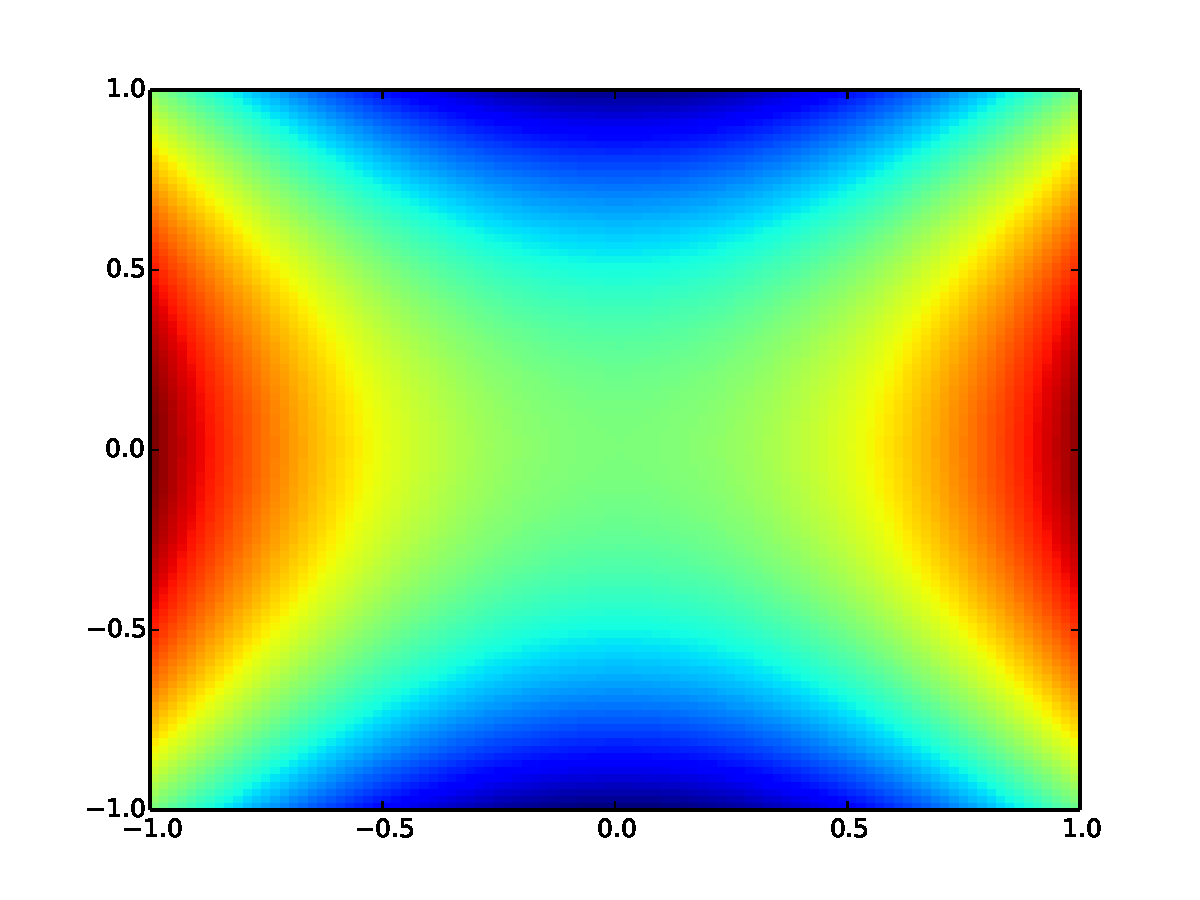
\includegraphics[width=\textwidth]{poly_color_plot_real}
\end{subfigure}
\begin{subfigure}{.49\textwidth}
\includegraphics[width=\textwidth]{poly_color_plot_imag}
\end{subfigure}
\caption{Color plots of the real and imaginary parts of $x^2 - 1$.}
\label{fig:poly_color_plot}
\end{figure}

\begin{figure}
\begin{subfigure}{.49\textwidth}
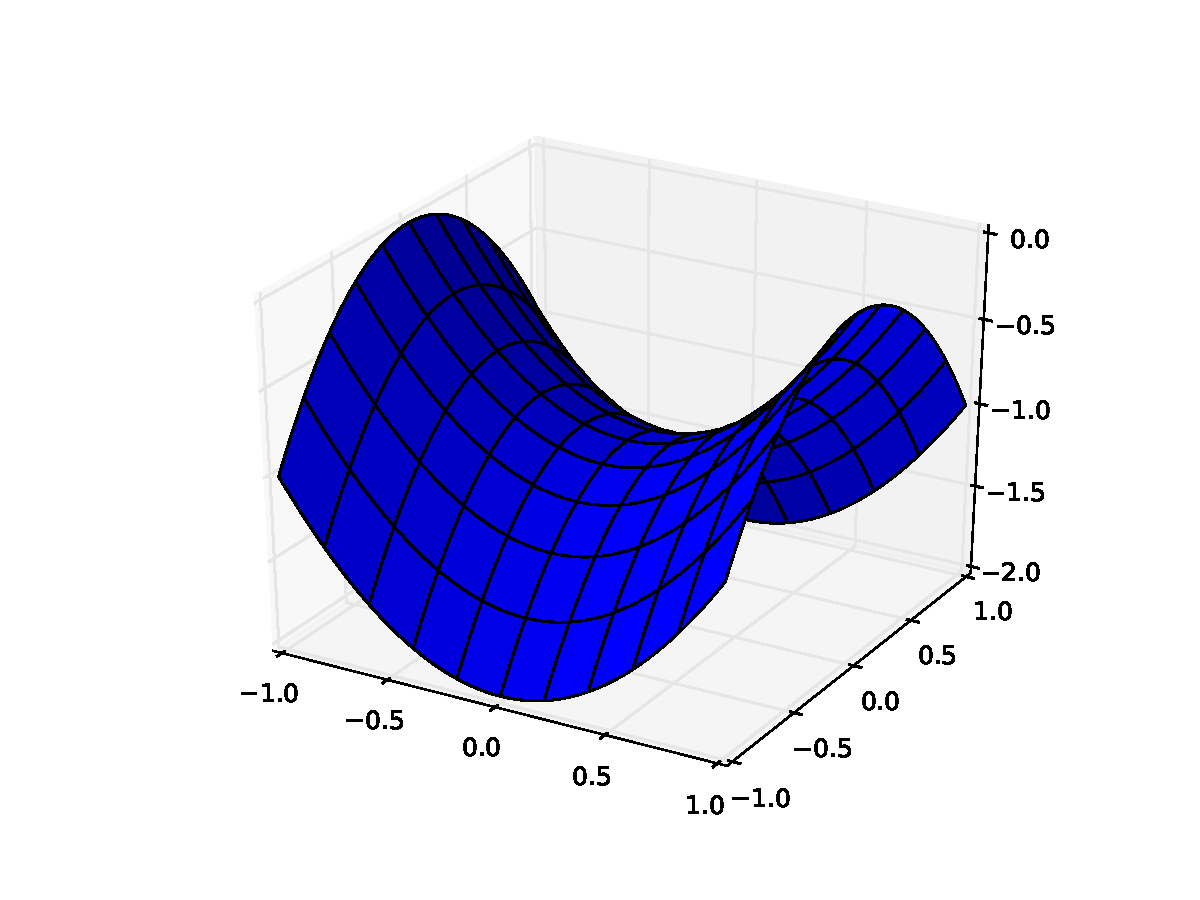
\includegraphics[width=\textwidth]{poly_surface_plot_real}
\end{subfigure}
\begin{subfigure}{.49\textwidth}
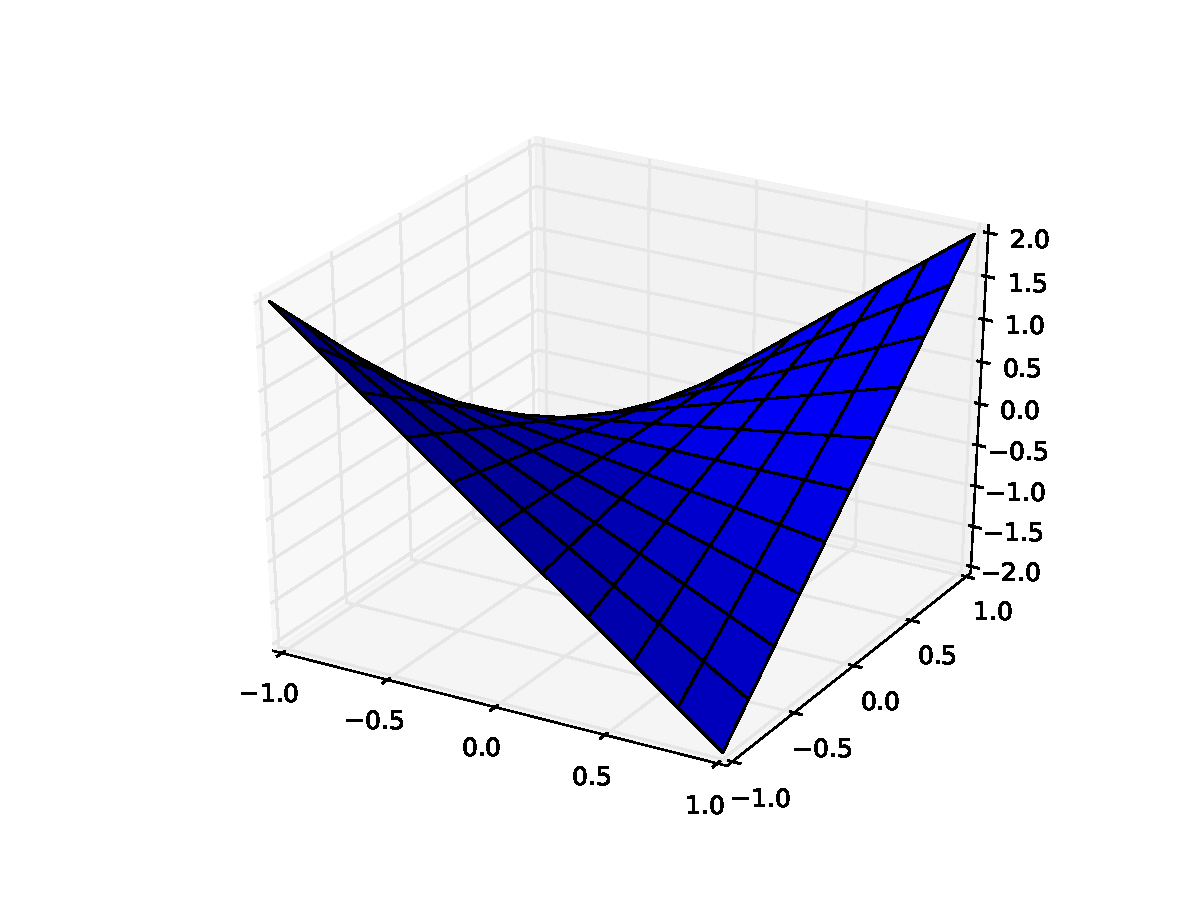
\includegraphics[width=\textwidth]{poly_surface_plot_imag}
\end{subfigure}
\caption{Surface plots of the real and imaginary parts of $x^2 - 1$.}
\label{fig:poly_surface_plot}
\end{figure}

\begin{problem}
Write three functions that graph the real part, the imaginary part, and both parts together of a given function 
Have each of them accept a callable funciton \li{f} and tuples \li{xlims} and \li{ylims} containing maximum and minimum values for the $x$ and $y$ axes.
Have the first function plot the real part of the complex valued function \li{f} on the region specified by \li{xlims} and \li{ylims} as surfaces in the 3D plane.
Have the second function plot the imaginary part.
Have the third function plot the real and imaginary part in on the same axis.

Use the third function you just wrote to plot both the real and imaginary parts of the polynomial $x^4 + 1$ on the domain $\left[-1, 1\right] \times \left[-1, 1\right]$.
Notice where the fourth roots of $-1$ lie on the plot, which roots you can obtain by calling \li{np.roots(np.poly1d([1,0,0,0,1]))}.
\end{problem}

\section*{Multi-Valued Functions}

Another important topic in Complex Analysis is the study of multiple valued functions.
These functions arise as we consider the inverses of functions that are not strictly one to one on the complex plane.
A classic example is $\sqrt{x}$, which may take two values for every nonzero point of the complex plane.

In the Real numbers we worked with functions like this by simply restricting their output on a certain domain.
We can do a similar thing in the Complex plane.
Loosely speaking, such a restriction is called a branch.
Computationally we restrict the output to a single portion of the actual possible values of the multifunction.
We call inverse functions that have multiple values like this ``multi-valued functions" or ``multifuctions."
We can still visualize the ``Riemann surfaces" of such multi-valued functions in the complex plane.
Figure \ref{fig:sqrt_riemann_surface} shows the Riemann surfaces for $\sqrt{z}$ in the complex plane.
Riemann surfaces are simple examples of manifolds.

\begin{figure}
\begin{subfigure}{.49\textwidth}
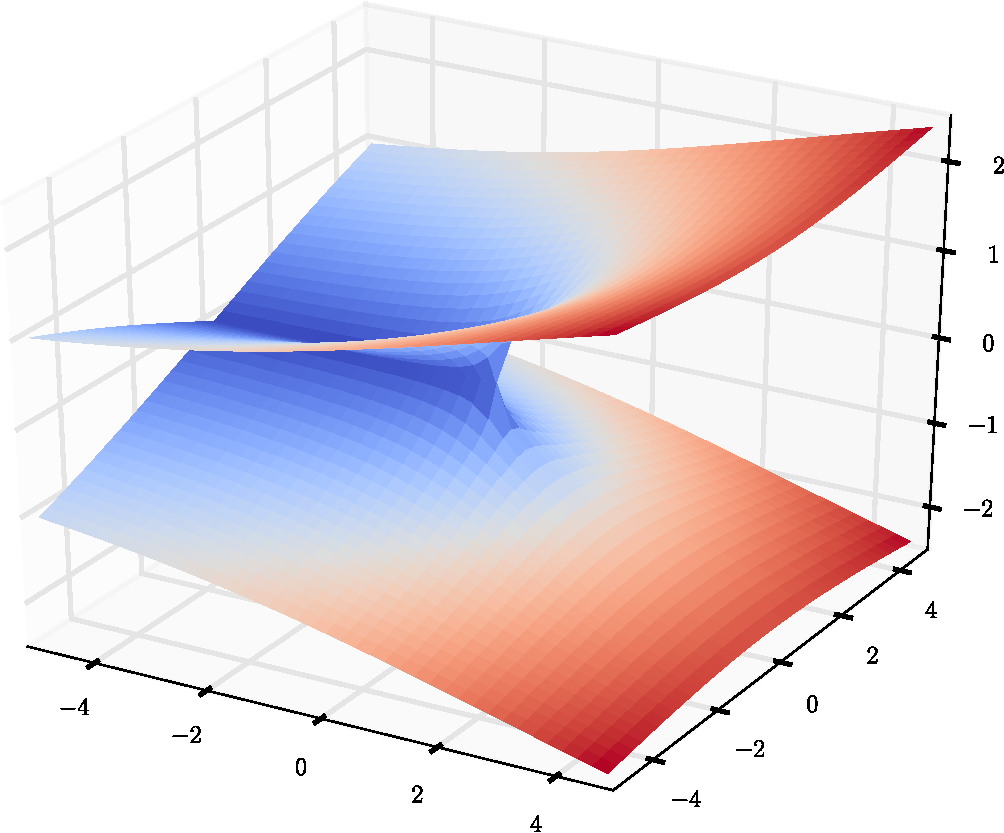
\includegraphics[width=\textwidth]{sqrt_riemann_surface_1}
\end{subfigure}
\begin{subfigure}{.49\textwidth}
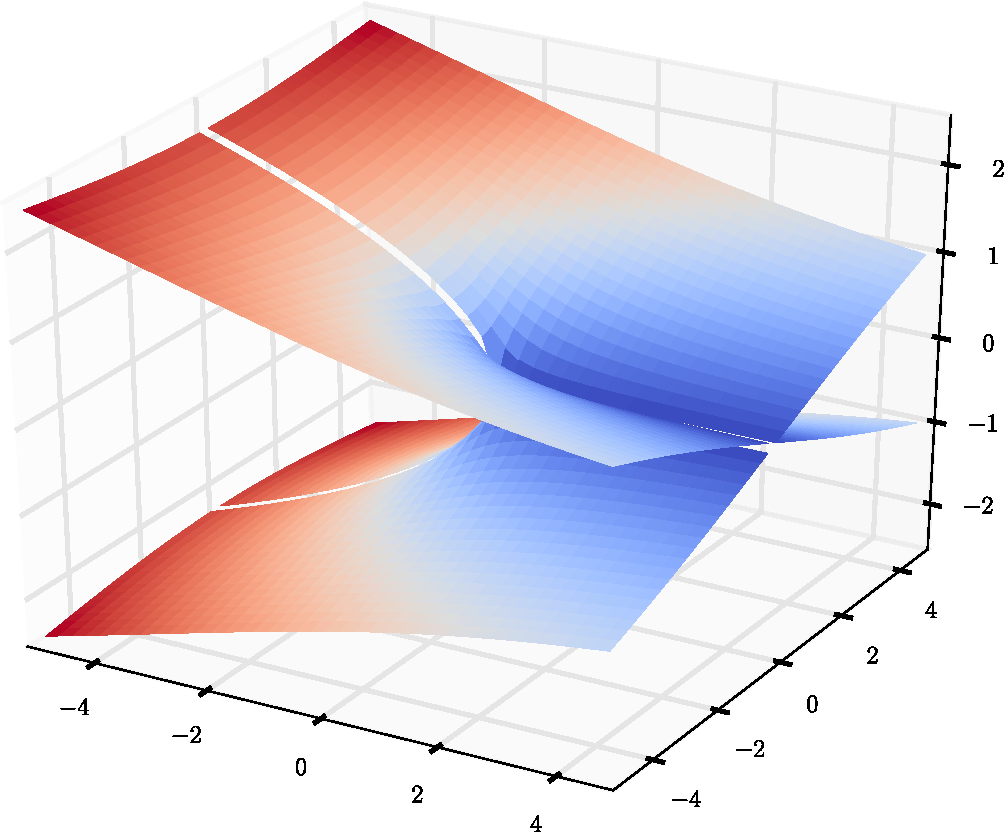
\includegraphics[width=\textwidth]{sqrt_riemann_surface_2}
\end{subfigure}
\caption{The real and imaginary parts of the function $\sqrt{z}$.}
\label{fig:sqrt_riemann_surface}
\end{figure}

These are some very basic examples.
Riemann surfaces can be very complex.
Another simple example is $\ln\left(z\right)$ which has a single value for the real part and infinitely many possible values for its imaginary part.
The Riemann surface for the imaginary part of $\ln\left(z\right)$ is shown in Figure \ref{fig:log_riemann_surface}.
Note that Figure \ref{fig:log_riemann_surface} is only a portion of the Riemann surface of the imaginary part of $\ln\left(z\right)$.
The full surface is, in actuality, an infinite spiral that repeats every $2\pi$.
This is because for any complex $z\neq 0$, we have $e^z=e^{z+2n\pi}$ where $n$ is any integer.

\begin{figure}
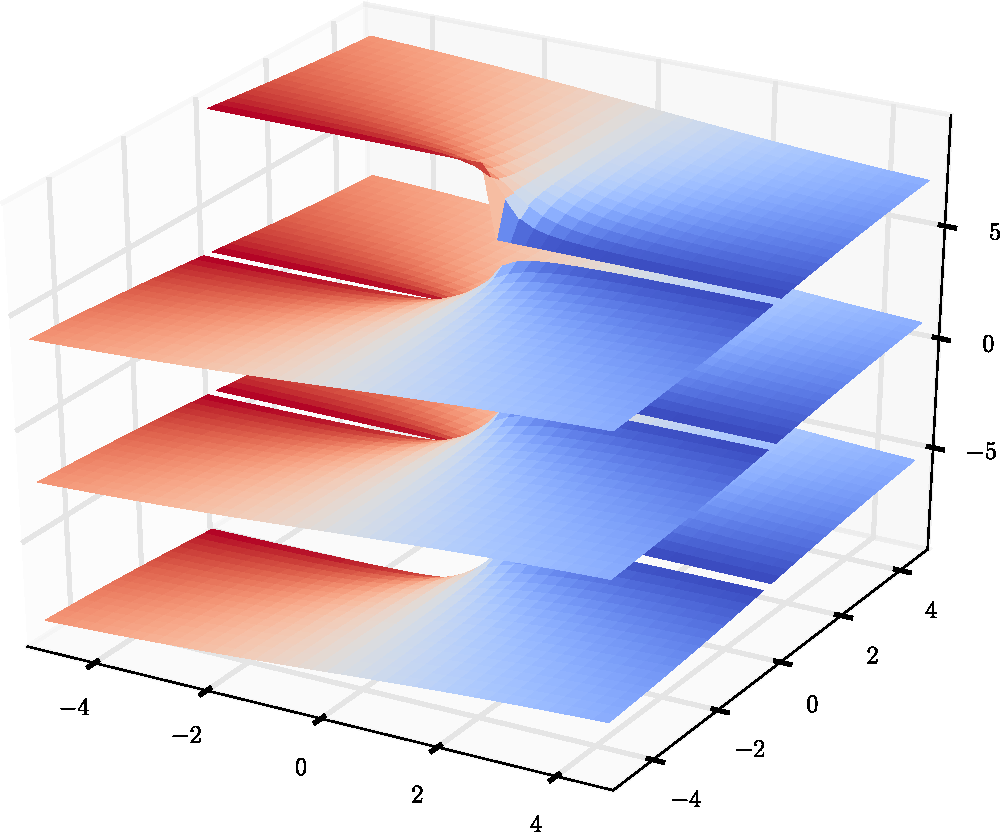
\includegraphics[width=\textwidth]{log_riemann_surface}
\caption{Riemann surface plot of a portion of the imaginary part of $\ln\left(z\right)$}
\label{fig:log_riemann_surface}
\end{figure}

Figure \ref{fig:arctan_riemann_surface} shows the real part of the riemann surface of $\arctan\left(z\right)$
All three of the functions we have plotted can be made analytic at almost any point, except at their singularities, but that depends on how we cut the domain to give it a single value.
When Integrating such functions, be careful about integrating across such cuts in the domain.

\begin{figure}
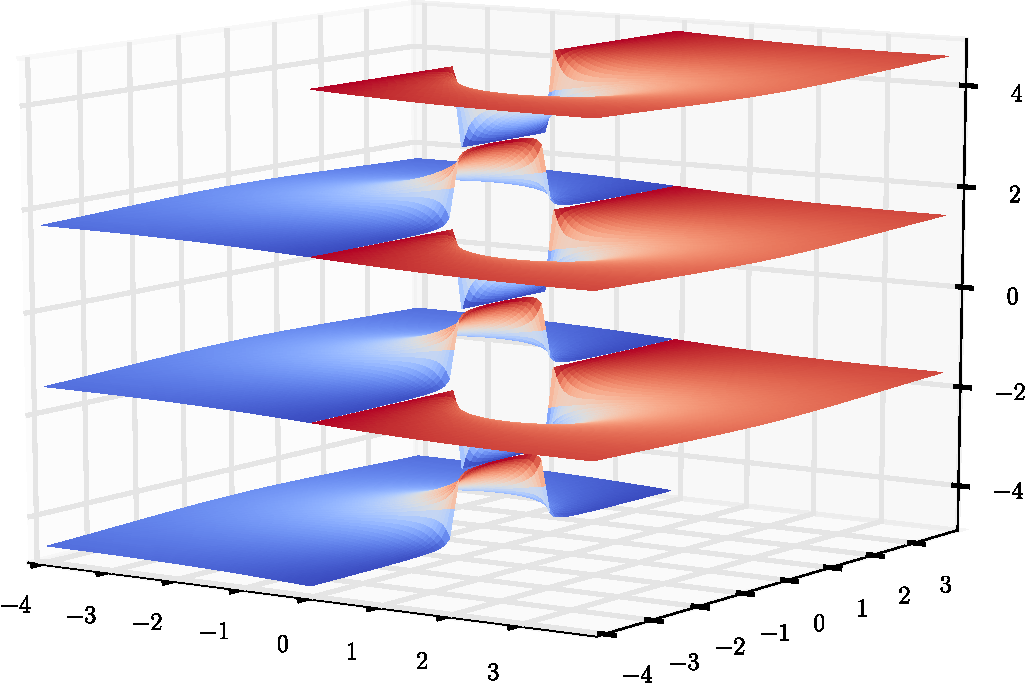
\includegraphics[width=\textwidth]{arctan_riemann_surface}
\caption{Even the Riemann surface of $\arctan(z)$ becomes increasingly complex.
This is a graph of a portion of the Riemann surface for the real part of $\arctan(z)$.}
\label{fig:arctan_riemann_surface}
\end{figure}

\begin{problem}
Write two functions, both accepting accept a natural number $n$.
Have one function plot the riemann surface for the real part $f(z)=\sqrt[n]{z}$ and the other plot the imaginary part.

Hint: Convert $z$ in $f(z)=\sqrt[n]{z}$ to polar form as $z=re^{\theta + 2k\pi}$
If you then plug this into $\sqrt[n]{z}$ the function takes the form
\[f(z)=\sqrt[n]{r} e^{i \frac{\theta + 2 \pi k}{n}}\]
Notice that here $f(z)$ has distinct values for $k = 0, 1, \dots, n-1$ a total of $n$ different values). Each value of $k$ corresponds to a different branch, which you can plot as $n$ separate surfaces.

If you use just one surface to plot each branch you will get erroneous vertical lines from jump discontinuities. Split each branch into two surfaces to get rid of these lines. You can investigate where the discontinuities occur by first plotting it as just one surface. The discontinuities happen at the same place for all $n$;
\end{problem}

\section*{Contour Integrals in the Complex Plane}

From multivariable calculus, you may recall that an integral may be taken along a path.
This is very similar to what we can be done in the complex plane.
Consider the function $f(z)$ on the complex plane.
Let $z=x+iy$ Let $u$ and $v$ be the real and imaginary parts of $f$ respectively.
We integrate $f$ along some contour $C$ in the complex plane, beginning at $z=a$ and ending at $z=b$.
This integral may be written
\[\int_c f(z)dz\]
Parameterizing $z$, we have
\[\int_a^b f(z(t))z'(t)dt=\]
Expanding into real and imaginary parts, we have
\[\int_a^b (u(z(t))x'(t)-v(z(t))y'(t))dt +i \int_a^b(v(z(t))x'(t)+u(z(t))y'(t))dt\]
We have now written this complex integral as the sum of two real valued integrals in $\mathbb{R}$.
Note that this implies that $\int_C f(z) dz$ may depend on the contour we choose and not just on the endpoints $a$ and $b$.

\begin{problem}
Write a function which takes a complex function $f(z)$, a contour parameterization $c(t)$ of a contour $c$, and the integration bounds on $t$ and returns the integral of $f$ along the contour $c$.
Use the numerical integration function \li{sympy.mpmath.quad} and the numerical derivative function \li{sympy.mpmath.diff} included in mpmath (which is, in turn, included as a submodule of sympy).
These functions already work for complex numbers.
To do something similar with the integration routines in SciPy, we would have to separate the function into real and imaginary parts, as is shown above.

Using the function you just defined, integrate the following functions along the following contours
\begin{itemize}
\item $\bar{z}$ counterclockwise along the unit ball starting and ending at $1$
\item $\bar{z}$ along a straight line from $0$ to $1+i$
\item $\bar{z}$ along the real axis from $0$ to $1$, then along the line from $1$ to $1+i$
\item $\bar{z}$ along the unit ball centered at $i$ from $0$ to $1+i$
\item $e^z$ counterclockwise along the unit ball starting and ending at $1$
\item $e^z$ along a straight line from $0$ to $1+i$
\item $e^z$ along the real axis from $0$ to $1$, then along the line from $1$ to $1+i$
\item $e^z$ along the unit ball centered at $i$ from $0$ to $1+i$
\end{itemize}
\end{problem}

Notice that, for a holomorphic function on a simply connected domain, the integrals from one point to another are not path dependent for any contours that lie within the domain.
An immediate consequence of the theorem is that for a complex function $f$, holomorphic on a simply connected domain $D$, and a contour $C$ lying entirely within $D$ which begins and ends at some point $a\in D$,
\[\int_C f(z)dz=0\]

The quadrature algorithms used in many of the integration algorithms work along a straight line between the integration bounds in the complex plane, so for holomorphic functions we should be able to use the integration function we wrote earlier.
For example, integrating $e^z$ from $-1-i$ to $1+i$ can be done numerically like this:
\begin{lstlisting}
from sympy import mpmath as mp
mp.quad(lambda z: mp.exp(z), (complex(-1, -1), complex(1, 1)))
\end{lstlisting}

\section*{The Cauchy Integral Formula}

Another major theorem in complex analysis is called Cauchy's Integral Formula (not to be confused with Cauchy's Integral Theorem).
It states that for a domain $D$ in the complex plane, containing some contour $C$ and the interior of $C$, for any $z_0$ in the interior of $C$,
\[f(z_0)=\frac{1}{2\pi i} \int_C \frac{f(z)}{z-z_0} dz\]

With more work, this theorem can be used to show that any function $f$ holomorphic on some domain $D$ is also infinitely differentiable on that domain.
In fact, the $n$th derivative of $f$ is given by the formula
\[f^{(n)}(z_0) = \frac{n!}{2\pi i} \int_C \frac{f(z)}{(z-z_0)^{n+1}} dz\]
This result is also important because it allows us to relate the value of $f$ on the inside of a contour to the value of $f$ on the contour itself.
In other words, the values of $f$ inside the contour depend only on the values of $f$ along the contour itself.
A related theorem (the Morera theorem) states that if some function $f$ is continuous on a domain $D$ and for every contour beginning and ending at the same point, the formula $\int_C f(z) dz = 0$ holds, then $f$ is holomorphic on $D$.

\begin{problem}
Using Cauchy's Integral Formula, write a python function which returns a callable function which evaluates a complex function $f$ along the interior of a contour $C$.
It should accept a callable function for the paramaterization of $C$, a callable function for the values of $f$ along $C$, and the bounds on the parameter used.
Assume in your function that $C$ begins and ends at the same point and that $f$ also begins and ends at the same value (so that $f$ is continous along $C$)
Try it out on simple functions like $e^x$ with complex values and compare what you get with what calling the functions normally gives you.
\end{problem}

Notice that in Cauchy's Integral Formula, we are integrating along a contour that begins and ends at the same point.
The function is also holomorphic at every point except $z_0$. At $z_0$ the integrand is undefined and has a singularity.
This integral around a singularity has some useful properties.
We will discuss these properties later on.
